\chapter{認証と接続 — パソコンとGitHubを安全につなぐ}

\section{この章で学ぶこと}

本章では、自分のパソコンとGitHubの間に「安全な通信路」を確立する方法を学びます。前章まででGitのインストールとGitHubアカウントの作成が完了しましたが、それだけではパソコンからGitHubにコードを送ったり、GitHubからコードを取得したりすることはできません。「このパソコンからの操作は、確かにこのGitHubアカウントの持ち主によるものである」という証明、つまり\textbf{認証}が必要です。

具体的には、以下の内容を学びます。

\begin{itemize}
  \item そもそも\textbf{なぜ認証が必要なのか}というセキュリティの基本的な考え方
  \item \textbf{SSH}、\textbf{HTTPS + Personal Access Token}、\textbf{GitHub CLI} という3つの接続方式の比較
  \item 最も広く推奨されている\textbf{SSH鍵による接続}の設定方法（公開鍵暗号の仕組みも含めて）
  \item HTTPS接続で使う\textbf{Personal Access Token（PAT）}の作成と管理
  \item コマンド一つで認証を完了できる\textbf{GitHub CLI}の活用
  \item コミットが本当に自分のものであることを証明する\textbf{GPG署名}
  \item 仕事用と個人用など、\textbf{複数アカウントの使い分け}方
\end{itemize}

認証の設定は、一度行えば日常的にやり直す必要はありません。しかし、仕組みを理解しておくことで、トラブルが起きたときに自分で対処できるようになります。少し難しく感じるかもしれませんが、一つずつ丁寧に進めていきましょう。

\section{なぜ認証が必要なのか}

GitHubにコードをアップロード（プッシュ）したり、プライベートリポジトリのコードをダウンロード（クローン）したりする操作を考えてみましょう。もし認証の仕組みがなかったらどうなるでしょうか。

誰でも他人のリポジトリにコードを書き込めてしまいます。悪意のある人がプロジェクトのコードを改ざんしたり、プライベートなコードを盗み見たりすることが可能になります。これは、鍵のかかっていない家に等しい状態です。

認証とは、「あなたが本当にあなたであること」を確認するプロセスです。GitHubにパソコンからアクセスする際、「このアクセスは、GitHubアカウント \cmd{tsubasa} の持ち主からのものです」ということを、何らかの方法で証明する必要があります。

以前は、ユーザー名とパスワードを入力するだけで認証できましたが、GitHubは2021年にパスワード認証を廃止しました。パスワードは盗まれやすく、使い回しのリスクもあるためです。現在は、より安全な認証方式のみが利用可能になっています。

\section{接続方式の比較}

GitHubとの接続方法は、大きく分けて3つあります。それぞれに特徴があり、状況に応じて使い分けることができます。

\begin{table}[htbp]
\centering
\begin{tabular}{lllll}
\hline
\textbf{方式} & \textbf{セキュリティ} & \textbf{手軽さ} & \textbf{推奨度} & \textbf{特徴} \\
\hline
\textbf{SSH鍵} & 非常に高い & 初回設定にやや手間 & 最も推奨 & 一度設定すれば認証不要 \\
\textbf{HTTPS + PAT} & 高い & トークン管理が必要 & 状況に応じて & ファイアウォール内でも可 \\
\textbf{GitHub CLI} & 非常に高い & 最も簡単 & 推奨 & コマンド一つで設定 \\
\hline
\end{tabular}
\end{table}

\textbf{初心者の方へのおすすめ}は、GitHub CLI（\cmd{gh}）を使う方法です。対話形式で質問に答えていくだけで、裏側でSSH鍵の生成やGitHubへの登録まで自動的に行ってくれます。

一方、\textbf{SSH鍵の仕組みを理解しておくこと}は、GitHub CLI を使う場合でも重要です。トラブルシューティングの際や、GitHub以外のGitサービス（GitLab、Bitbucket など）を使う際にも必ず役立ちます。そのため、本章ではSSH鍵の解説を最も詳しく行います。

\section{SSH鍵による接続（推奨）}

\subsection{公開鍵暗号の仕組み — 南京錠のたとえ}

SSH鍵を理解するために、まず「公開鍵暗号」という仕組みを平易に説明します。

公開鍵暗号は、2つの鍵を使う暗号方式です。たとえ話で説明しましょう。

あなたが誰かに秘密のメッセージを送りたいとします。従来の方法（共通鍵暗号）では、一つの鍵で箱を施錠し、同じ鍵で開錠します。しかし、その鍵をどうやって相手に安全に渡すかという問題があります。鍵を配送中に盗まれたら、メッセージも読まれてしまいます。

公開鍵暗号は、この問題を巧妙に解決します。仕組みはこうです。

\begin{enumerate}
  \item あなたは「\textbf{南京錠}」（公開鍵）と「\textbf{南京錠を開ける鍵}」（秘密鍵）のペアを作ります
  \item 南京錠（公開鍵）は世界中にばらまいても構いません。誰でも持って行ってOKです
  \item メッセージを送りたい人は、あなたの南京錠で箱を施錠して送ります
  \item その箱を開けられるのは、南京錠を開ける鍵（秘密鍵）を持っているあなただけです
\end{enumerate}

SSH鍵もこれと同じ原理です。

\begin{itemize}
  \item \textbf{公開鍵}（\cmd{id\_ed25519.pub}）：GitHubに登録します。「南京錠」に相当します
  \item \textbf{秘密鍵}（\cmd{id\_ed25519}）：自分のパソコンに保管します。「南京錠を開ける鍵」に相当します。\textbf{絶対に他人に渡してはいけません}
\end{itemize}

\begin{figure}[htbp]
\centering
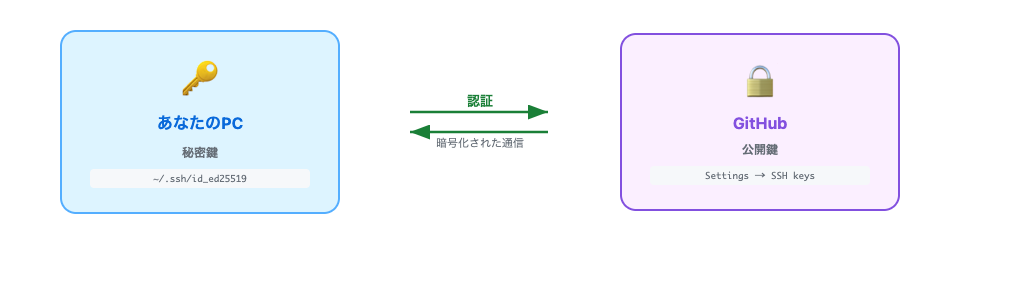
\includegraphics[width=0.9\textwidth]{images/diagram-ssh-auth.png}
\end{figure}

GitHubにアクセスするとき、GitHubは「この公開鍵に対応する秘密鍵を持っていますか？」と確認します。あなたのパソコンが秘密鍵を使って正しく応答できれば、「本人である」と認められます。秘密鍵そのものがネットワーク上を流れることはないため、非常に安全です。

\subsection{SSH鍵の生成}

それでは、実際にSSH鍵を生成しましょう。ターミナルを開いて次のコマンドを実行します。

\begin{lstlisting}[language=bash]
ssh-keygen -t ed25519 -C "your-email@example.com"
\end{lstlisting}

各オプションの意味を説明します。

\begin{itemize}
  \item \cmd{-t ed25519}：鍵の種類（アルゴリズム）を指定しています。Ed25519 は現在最も推奨されているアルゴリズムで、RSAよりも短い鍵長で同等以上のセキュリティを提供します。古い環境で Ed25519 がサポートされていない場合は、\cmd{-t rsa -b 4096} を使ってください。
  \item \cmd{-C "your-email@example.com"}：コメントを付加します。このコメントは鍵の識別に使われるもので、認証には影響しません。GitHubに登録したメールアドレスを入れておくのが慣例です。
\end{itemize}

コマンドを実行すると、いくつかの質問が表示されます。

\begin{lstlisting}[language={}]
Generating public/private ed25519 key pair.
Enter file in which to save the key (/Users/you/.ssh/id_ed25519):
\end{lstlisting}

鍵の保存場所を聞かれています。特に理由がなければ、そのまま Enter キーを押してデフォルトの場所に保存してください。

\begin{lstlisting}[language={}]
Enter passphrase (empty for no passphrase):
Enter same passphrase again:
\end{lstlisting}

次に\textbf{パスフレーズ}の設定を求められます。パスフレーズは、秘密鍵に追加のパスワードをかけるものです。パスフレーズを設定しておくと、万が一パソコンが盗まれたり、秘密鍵ファイルが流出したりしても、パスフレーズを知らなければ鍵を使うことができません。

セキュリティの観点から、パスフレーズの設定を強くおすすめします。後述するSSHエージェントを使えば、パスフレーズを毎回手入力する手間も省けます。

鍵の生成が完了すると、\cmd{\textasciitilde/.ssh/} ディレクトリに以下の2つのファイルが作成されます。

\begin{itemize}
  \item \cmd{id\_ed25519}：秘密鍵。このファイルは絶対に他人と共有しないでください。
  \item \cmd{id\_ed25519.pub}：公開鍵。このファイルの内容をGitHubに登録します。
\end{itemize}

\subsection{SSHエージェントに鍵を登録する}

SSHエージェントは、秘密鍵をメモリ上に保持してくれるプログラムです。エージェントに鍵を登録しておくと、SSH接続のたびにパスフレーズを入力する必要がなくなります。自動車でいえば、エンジンをかけるたびにキーを回す代わりに、スマートキーで自動的にエンジンがかかるようなイメージです。

まず、SSHエージェントをバックグラウンドで起動します。

\begin{lstlisting}[language=bash]
eval "$(ssh-agent -s)"
\end{lstlisting}

\cmd{Agent pid 12345} のような出力が表示されれば、エージェントが起動しています。

\textbf{macOSの場合}は、SSH設定ファイルを作成（または編集）して、Keychainとの連携を設定します。

\begin{lstlisting}[language=bash]
cat >> ~/.ssh/config << 'EOF'
Host github.com
  AddKeysToAgent yes
  UseKeychain yes
  IdentityFile ~/.ssh/id_ed25519
EOF
\end{lstlisting}

この設定の意味を解説します。

\begin{itemize}
  \item \cmd{Host github.com}：以下の設定が \cmd{github.com} への接続時に適用されることを示します
  \item \cmd{AddKeysToAgent yes}：鍵を使用する際に自動的にSSHエージェントに追加します
  \item \cmd{UseKeychain yes}：macOSのKeychain（パスワード管理機能）にパスフレーズを保存します。これにより、パソコンを再起動してもパスフレーズの再入力が不要になります
  \item \cmd{IdentityFile \textasciitilde/.ssh/id\_ed25519}：使用する秘密鍵のファイルパスを指定します
\end{itemize}

次に、鍵をエージェントに追加します。

\begin{lstlisting}[language=bash]
# macOSの場合
ssh-add --apple-use-keychain ~/.ssh/id_ed25519

# Linuxの場合
ssh-add ~/.ssh/id_ed25519
\end{lstlisting}

パスフレーズを設定している場合、ここで入力を求められます。一度入力すれば、以降はエージェントが自動的に処理してくれます。

\subsection{公開鍵をGitHubに登録する}

生成した公開鍵をGitHubに登録します。まず、公開鍵の内容をクリップボードにコピーします。

\begin{lstlisting}[language=bash]
# macOSの場合
pbcopy < ~/.ssh/id_ed25519.pub

# Linuxの場合（xclipがインストールされている場合）
xclip -selection clipboard < ~/.ssh/id_ed25519.pub

# または、内容を表示して手動でコピー
cat ~/.ssh/id_ed25519.pub
\end{lstlisting}

公開鍵は \cmd{ssh-ed25519 AAAA...} で始まる1行のテキストです。

次に、GitHubのWebサイトで以下の操作を行います。

\begin{enumerate}
  \item GitHubにログインし、右上のアイコンから \textbf{Settings} を開きます
  \item 左側のメニューから \textbf{SSH and GPG keys} を選択します
  \item 「\textbf{New SSH key}」ボタンをクリックします
  \item \textbf{Title}：この鍵を識別するための名前を入力します。「MacBook Pro 2024」や「自宅デスクトップ」など、どのパソコンの鍵かがわかる名前にしましょう
  \item \textbf{Key type}：「Authentication Key」を選択します
  \item \textbf{Key}：コピーした公開鍵を貼り付けます
  \item 「\textbf{Add SSH key}」をクリックします
\end{enumerate}

\begin{figure}[htbp]
\centering
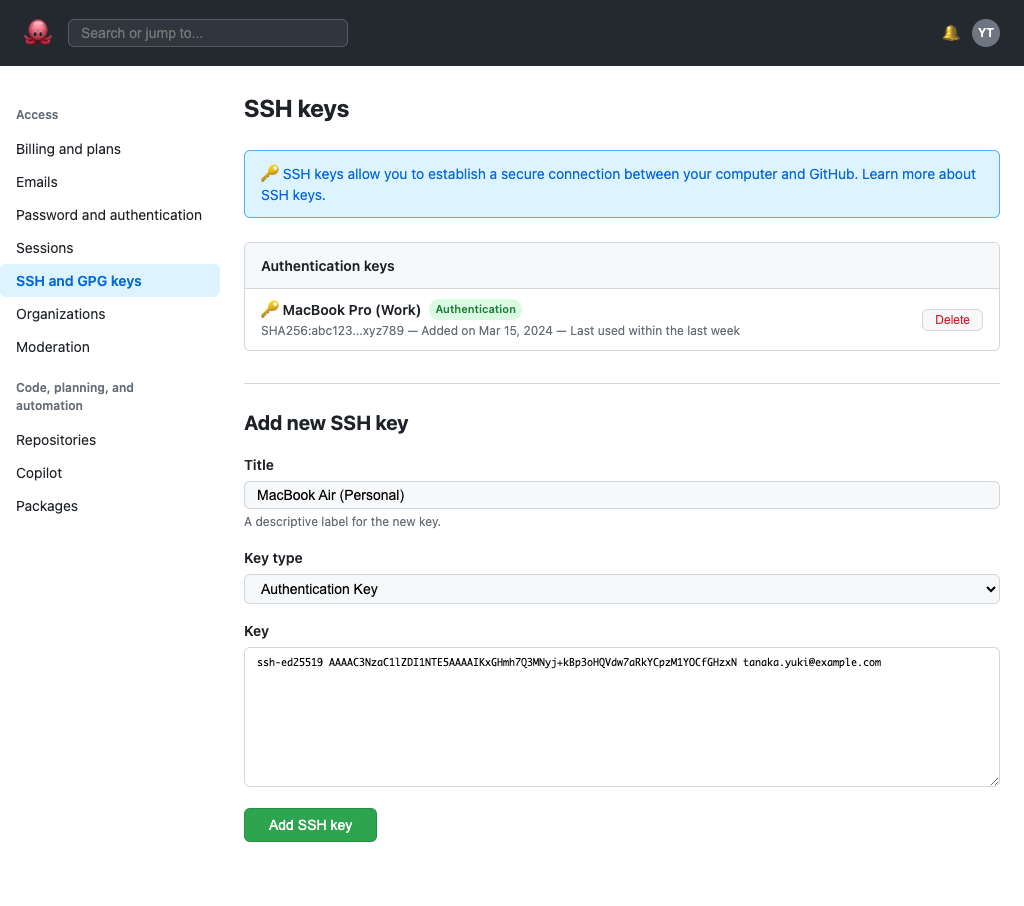
\includegraphics[width=0.95\textwidth]{images/ssh-key-add.png}
\caption{SSH鍵の追加画面}
\end{figure}

GitHubのパスワード入力を求められることがありますが、これはセキュリティ上の確認です。

\subsection{接続テスト}

設定が正しくできたかどうかを確認しましょう。

\begin{lstlisting}[language=bash]
ssh -T git@github.com
\end{lstlisting}

初めて接続する場合、以下のようなメッセージが表示されることがあります。

\begin{lstlisting}[language={}]
The authenticity of host 'github.com (20.27.177.113)' can't be established.
ED25519 key fingerprint is SHA256:+DiY3wvvSqA3npr5lFzhzg6hcJkiGk....
Are you sure you want to continue connecting (yes/no/[fingerprint])?
\end{lstlisting}

これは「このサーバーに初めて接続しますが、本当に接続しますか？」という確認です。\cmd{yes} と入力してください。GitHubのフィンガープリント（サーバーの指紋）は、GitHubの公式ドキュメントで公開されていますので、心配な場合は照合することもできます。

接続に成功すると、以下のメッセージが表示されます。

\begin{lstlisting}[language={}]
Hi username! You've been successfully authenticated, but GitHub does not provide shell access.
\end{lstlisting}

「shell access」（シェルへのアクセス）は提供されないと書かれていますが、これは正常です。GitHubはGitリポジトリのホスティングサービスであり、サーバーにログインして操作するサービスではないためです。認証自体は成功しています。

\subsection{SSH接続でリポジトリを操作する}

SSH接続が確立できたら、以降はSSH形式のURLを使ってリポジトリを操作します。

\begin{lstlisting}[language=bash]
# SSHのURLでリポジトリをクローン
git clone git@github.com:username/repo.git

# 既存リポジトリのリモートURLをSSHに変更する場合
git remote set-url origin git@github.com:username/repo.git
\end{lstlisting}

SSH形式のURLは \cmd{git@github.com:ユーザー名/リポジトリ名.git} という形式です。HTTPS形式の \cmd{https://github.com/...} とは異なることに注意してください。GitHubのリポジトリページで「Code」ボタンをクリックすると、「SSH」タブでこのURLを確認できます。

\section{HTTPS + Personal Access Token}

SSH鍵の代わりに、HTTPS接続と Personal Access Token（PAT）を使う方法もあります。企業のネットワーク環境ではSSHポート（22番）がファイアウォールでブロックされていることがあり、その場合はHTTPS（443番ポート）を使うこの方式が有効です。

\subsection{Personal Access Token（PAT）とは}

PATは、パスワードの代わりに使用する「トークン（文字列）」です。GitHubのパスワードとは別に生成され、有効期限や権限の範囲を細かく設定できます。パスワードがアカウント全体の「万能鍵」だとすれば、PATは「特定の部屋だけ開けられる鍵」のようなものです。

\subsection{PATの作成手順}

\begin{enumerate}
  \item GitHubにログインし、右上のアイコンから \textbf{Settings} を開きます
  \item 左側メニューの一番下にある \textbf{Developer settings} をクリックします
  \item \textbf{Personal access tokens} → \textbf{Tokens (classic)} を選択します
  \item 「\textbf{Generate new token (classic)}」をクリックします
\end{enumerate}

\begin{figure}[htbp]
\centering
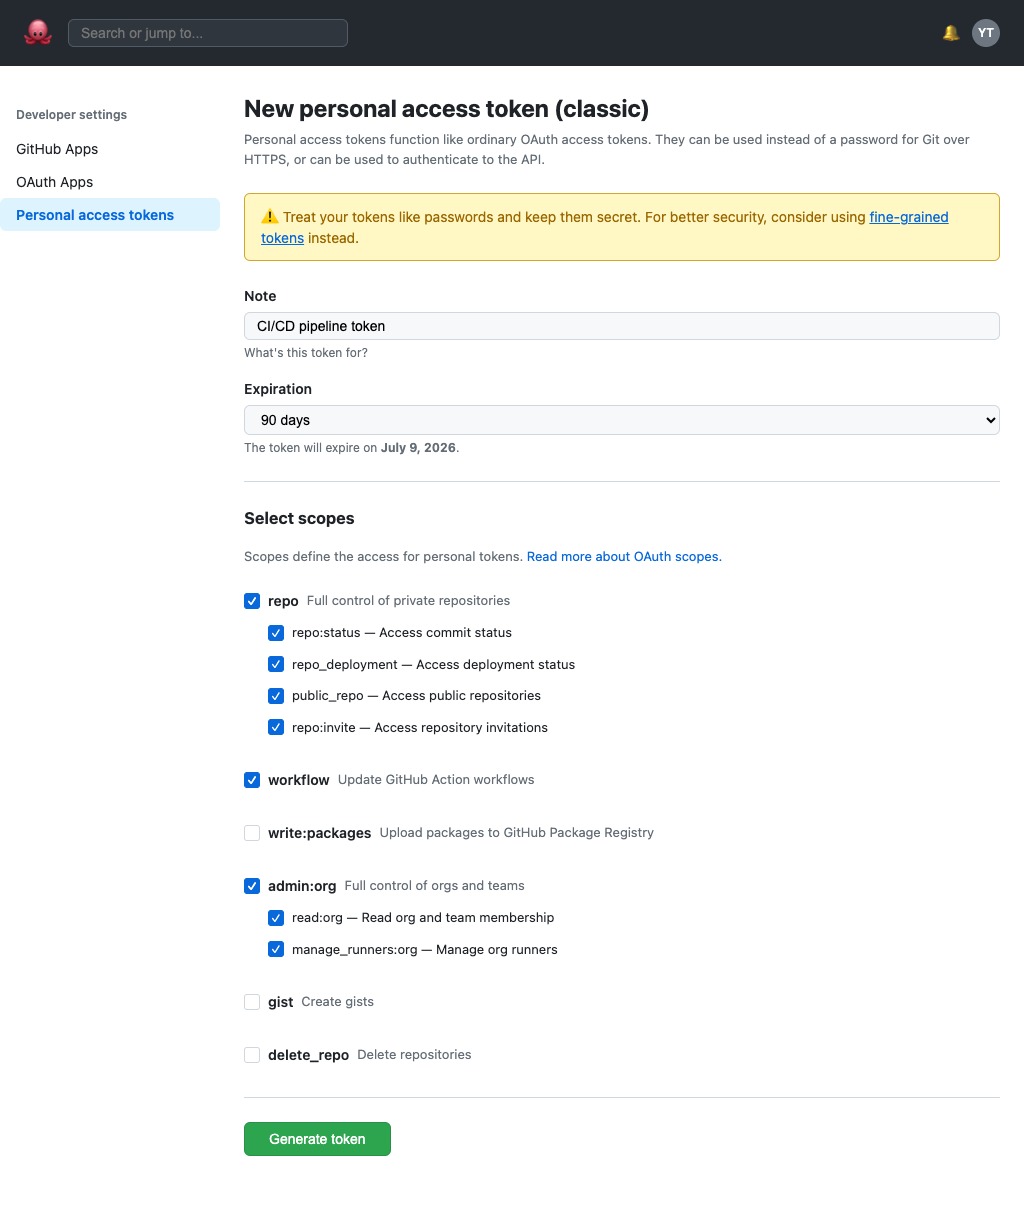
\includegraphics[width=0.95\textwidth]{images/pat-create.png}
\caption{PAT作成画面}
\end{figure}

以下の項目を設定します。

\textbf{Note（メモ）}：このトークンの用途を書きます。「MacBook 開発用」「CI/CD パイプライン用」など、後から見て何のために作ったトークンかがわかる名前にしてください。

\textbf{Expiration（有効期限）}：トークンの有効期間を設定します。90日程度が推奨されます。有効期限を設定しないこともできますが、セキュリティの観点からおすすめしません。期限が切れたら、新しいトークンを生成して差し替えます。

\textbf{Scopes（スコープ = 権限範囲）}：このトークンにどの操作を許可するかを選択します。

\subsection{スコープの選び方}

\begin{table}[htbp]
\centering
\begin{tabular}{llp{7cm}}
\hline
\textbf{スコープ} & \textbf{用途} & \textbf{必要な場面} \\
\hline
\cmd{repo} & リポジトリの読み書き & ほぼ必須。プライベートリポジトリへのアクセスに必要です \\
\cmd{workflow} & GitHub Actionsワークフローの管理 & CI/CDを使う場合に必要です \\
\cmd{admin:org} & Organization（組織）の管理 & 組織のメンバー管理などを行う場合 \\
\cmd{gist} & Gistの作成・編集 & Gistを使う場合のみ \\
\cmd{delete\_repo} & リポジトリの削除 & 通常は不要です。付与しないことを推奨 \\
\hline
\end{tabular}
\end{table}

\textbf{最小権限の原則}に従い、必要最低限のスコープだけを選択してください。日常的な開発作業であれば、\cmd{repo} と \cmd{workflow} の2つで十分です。

「\textbf{Generate token}」をクリックすると、トークンが表示されます。\textbf{このトークンは一度しか表示されません}。画面を閉じるとニ度と確認できなくなるため、必ずコピーしてパスワードマネージャーなどの安全な場所に保存してください。

\subsection{PATを使ったリポジトリ操作}

\begin{lstlisting}[language=bash]
# HTTPS URLでクローン
git clone https://github.com/username/repo.git
\end{lstlisting}

ユーザー名とパスワードを聞かれたら、パスワードの代わりにPATを入力します。

\subsection{認証情報の保存（毎回入力しなくて済むように）}

HTTPS接続では、操作のたびにユーザー名とトークンの入力を求められることがあります。これを省略するために、OSの認証情報管理機能を活用しましょう。

\begin{lstlisting}[language=bash]
# macOSの場合：Keychainに保存
git config --global credential.helper osxkeychain

# Windowsの場合：Windows Credential Managerに保存
git config --global credential.helper wincred

# Linuxの場合：一定時間メモリに保存（秒数で指定、以下は1時間）
git config --global credential.helper 'cache --timeout=3600'
\end{lstlisting}

macOSの \cmd{osxkeychain} と Windowsの \cmd{wincred} は、OS内蔵のパスワード管理機能に認証情報を安全に保存します。一度入力すれば、以降は自動的に認証が行われます。

Linuxの \cmd{cache} は、メモリ上に一時的に保存する方式で、指定した秒数が経過すると認証情報は消えます。永続的に保存したい場合は \cmd{store} ヘルパーもありますが、トークンが平文（暗号化なし）でファイルに保存されるため、セキュリティ上のリスクがあります。可能であれば、\cmd{libsecret} や \cmd{pass} などの暗号化された認証情報ストアの利用を検討してください。

\subsection{Fine-grained PAT（きめ細かいPAT）}

GitHubは、従来のPAT（Classic）に加えて、\textbf{Fine-grained PAT}（きめ細かいPAT）という新しい方式も提供しています。

Fine-grained PATでは、以下のようなより詳細な権限制御が可能です。

\begin{itemize}
  \item \textbf{リポジトリ単位}で権限を設定できる（特定のリポジトリだけにアクセスを限定）
  \item \textbf{読み取りのみ}・\textbf{読み書き}などの粒度で権限を設定できる
  \item 組織のセキュリティポリシーに準拠したトークンを作成できる
\end{itemize}

作成は \textbf{Developer settings → Personal access tokens → Fine-grained tokens} から行います。より安全なトークン管理が可能なため、新規にトークンを作成する場合はFine-grained PATの使用を検討してみてください。

\section{GitHub CLI}

GitHub CLI（コマンド名：\cmd{gh}）は、GitHubが公式に提供するコマンドラインツールです。認証の設定をはじめ、リポジトリの作成、プルリクエストの操作、Issueの管理など、GitHub上のほぼすべての操作をターミナルから行えます。

認証に関して言えば、GitHub CLI は最も簡単な方法です。対話形式で質問に答えていくだけで、SSH鍵の生成からGitHubへの登録までを自動的に行ってくれます。

\subsection{インストール}

\begin{lstlisting}[language=bash]
# macOS（Homebrew）
brew install gh

# Windows（winget）
winget install --id GitHub.cli

# Linux（Debian/Ubuntu）
sudo apt install gh

# Linux（Fedora）
sudo dnf install gh
\end{lstlisting}

\subsection{認証の設定}

インストールが完了したら、次のコマンドで認証を開始します。

\begin{lstlisting}[language=bash]
gh auth login
\end{lstlisting}

対話形式でいくつかの質問が表示されます。

\begin{lstlisting}[language={}]
? What account do you want to log into?  GitHub.com
? What is your preferred protocol for Git operations?  SSH
? Generate a new SSH key to add to your GitHub account?  Yes
? Title for your SSH key:  MacBook Pro
? How would you like to authenticate GitHub CLI?  Login with a web browser
\end{lstlisting}

各質問の意味を解説します。

\begin{itemize}
  \item \textbf{アカウントの種類}：\cmd{GitHub.com}（通常のGitHub）か \cmd{GitHub Enterprise Server}（企業向け自社ホスト版）かを選びます。ほとんどの場合は \cmd{GitHub.com} です。
  \item \textbf{Git操作のプロトコル}：\cmd{SSH} を選択することをおすすめします。この選択により、GitHub CLI がSSH鍵の設定も併せて行ってくれます。
  \item \textbf{SSH鍵の生成}：まだSSH鍵を作成していなければ \cmd{Yes} を選びます。すでに4.4節の手順で鍵を作成済みの場合は、既存の鍵を使うことも可能です。
  \item \textbf{SSH鍵のタイトル}：GitHubに登録する際の識別名です。どのパソコンの鍵かがわかる名前を付けましょう。
  \item \textbf{認証方法}：\cmd{Login with a web browser} を選ぶと、ブラウザが自動的に開き、GitHubのログインページが表示されます。ターミナルに表示されるコードをブラウザに入力して認証を完了してください。
\end{itemize}

\begin{figure}[htbp]
\centering
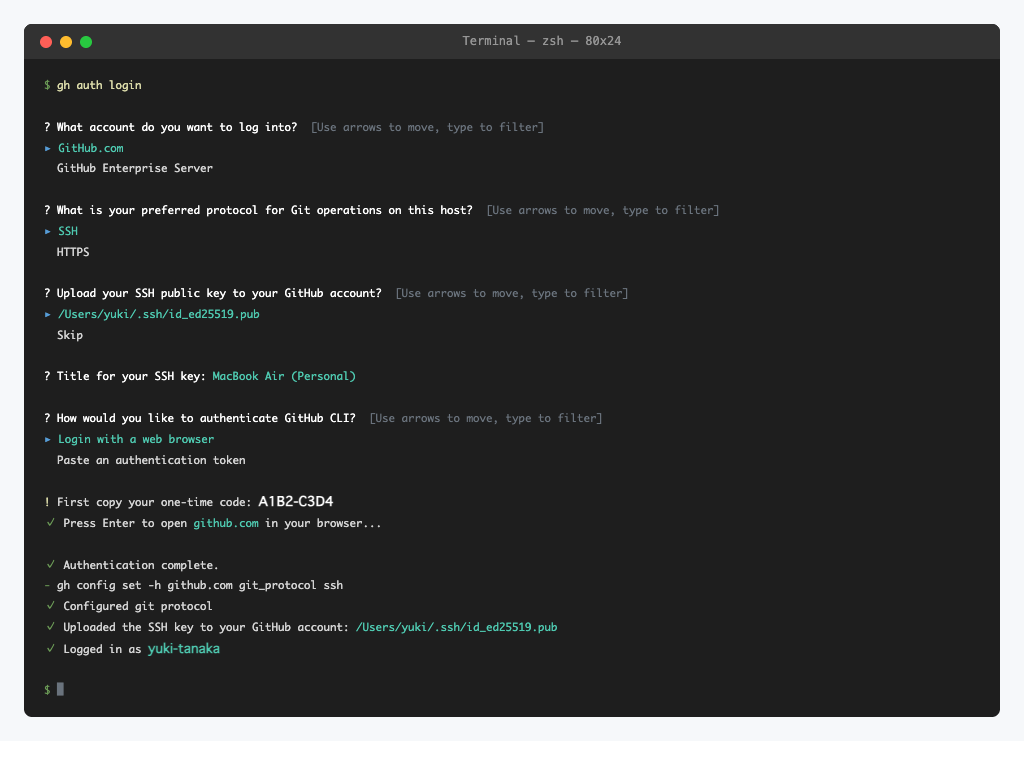
\includegraphics[width=0.95\textwidth]{images/gh-auth-login.png}
\caption{gh auth login の対話画面}
\end{figure}

ブラウザでの認証が完了すると、ターミナルに認証成功のメッセージが表示されます。これで設定は完了です。

\subsection{認証状態の確認}

現在の認証状態を確認するには、次のコマンドを使います。

\begin{lstlisting}[language=bash]
gh auth status
\end{lstlisting}

出力例：

\begin{lstlisting}[language={}]
github.com
  Logged in to github.com account username (keyring)
  - Active account: true
  - Git operations protocol: ssh
  - Token: gho_****
  - Token scopes: 'admin:org', 'gist', 'repo', 'workflow'
\end{lstlisting}

この出力から、ログインしているアカウント、Git操作で使われるプロトコル、トークンのスコープなどを確認できます。もし認証に問題がある場合は、\cmd{gh auth login} を再度実行して設定をやり直すことができます。

\section{GPG署名 — コミットの本人証明}

\subsection{なぜ署名が必要なのか}

第2章で \cmd{user.name} と \cmd{user.email} を設定しましたが、実はこの情報は\textbf{誰でも自由に設定できます}。極端な話、他人のユーザー名とメールアドレスを設定してコミットすることも技術的には可能です。つまり、コミットの「著者情報」だけでは、そのコミットが本当にその人によるものかどうかを保証できないのです。

GPG署名は、この問題を解決します。GPG（GNU Privacy Guard）という暗号ツールを使ってコミットに電子署名を付与することで、「このコミットは確かに私が作成したものです」という暗号的な証明を提供します。

GPG署名されたコミットは、GitHub上で「\textbf{Verified}」（検証済み）という緑色のバッジが表示されます。このバッジがあるコミットは、GitHubに登録されたGPG公開鍵と照合され、本人によるものであることが確認済みです。

\begin{figure}[htbp]
\centering
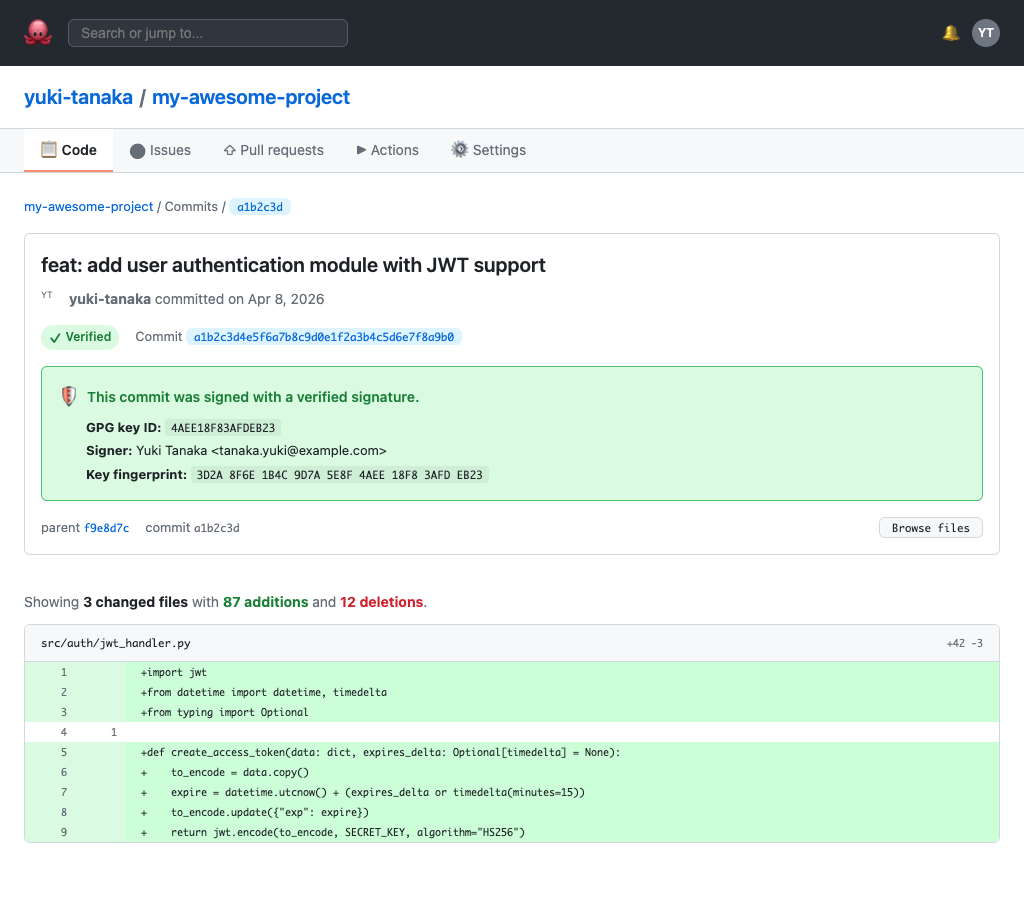
\includegraphics[width=0.95\textwidth]{images/verified-commit.png}
\caption{Verifiedバッジ付きコミット}
\end{figure}

オープンソースプロジェクトやセキュリティが重視される環境では、GPG署名が求められることがあります。必須ではありませんが、設定しておくとコミットの信頼性が高まります。

\subsection{GPG鍵の生成}

まず、GPGをインストールします。

\begin{lstlisting}[language=bash]
# macOS（Homebrew）
brew install gnupg

# Linux（Ubuntu/Debian）
sudo apt install gnupg

# Windows：Git for Windows に同梱されている場合があります
\end{lstlisting}

次に、GPG鍵を生成します。

\begin{lstlisting}[language=bash]
gpg --full-generate-key
\end{lstlisting}

いくつかの質問が表示されます。

\begin{itemize}
  \item \textbf{鍵の種類}：\cmd{RSA and RSA}（デフォルト）を選択します
  \item \textbf{鍵のビット数}：\cmd{4096} を入力します。2048ビットでも十分ですが、4096ビットにしておくとより長期間安全です
  \item \textbf{有効期限}：\cmd{0}（無期限）でも構いませんが、セキュリティを重視するなら1〜2年に設定し、期限が来たら更新することも検討してください
  \item \textbf{名前}：GitHubの表示名と一致させてください
  \item \textbf{メールアドレス}：GitHubに登録したメールアドレス（またはnoreplyアドレス）を入力してください
  \item \textbf{パスフレーズ}：GPG鍵を保護するパスフレーズを設定します
\end{itemize}

\subsection{GitHubにGPG鍵を登録する}

まず、生成した鍵のIDを確認します。

\begin{lstlisting}[language=bash]
gpg --list-secret-keys --keyid-format=long
\end{lstlisting}

出力例：

\begin{lstlisting}[language={}]
/Users/you/.gnupg/pubring.kbx
------------------------------
sec   rsa4096/3AA5C34371567BD2 2024-01-01 [SC]
      A1B2C3D4E5F6G7H8I9J0K1L2M3N4O5P6Q7R8S9T0
uid                 [ultimate] Your Name <your-email@example.com>
ssb   rsa4096/1234567890ABCDEF 2024-01-01 [E]
\end{lstlisting}

\cmd{sec} 行の \cmd{rsa4096/} の後に続く \cmd{3AA5C34371567BD2} が鍵IDです。

次に、公開鍵をテキスト形式でエクスポートします。

\begin{lstlisting}[language=bash]
gpg --armor --export 3AA5C34371567BD2
\end{lstlisting}

\cmd{-----BEGIN PGP PUBLIC KEY BLOCK-----} から \cmd{-----END PGP PUBLIC KEY BLOCK-----} までの全文をコピーし、GitHubに登録します。

\begin{enumerate}
  \item GitHub → Settings → \textbf{SSH and GPG keys} を開きます
  \item 「\textbf{New GPG key}」ボタンをクリックします
  \item コピーした公開鍵の全文を貼り付けます
  \item 「\textbf{Add GPG key}」をクリックします
\end{enumerate}

\subsection{Gitで署名を有効化する}

最後に、Gitがコミット時に自動的にGPG署名を付与するように設定します。

\begin{lstlisting}[language=bash]
# 使用するGPG鍵のIDを指定
git config --global user.signingkey 3AA5C34371567BD2

# すべてのコミットを自動的に署名する
git config --global commit.gpgsign true

# GPGプログラムのパスを指定（macOSで必要な場合）
git config --global gpg.program gpg
\end{lstlisting}

\cmd{commit.gpgsign true} を設定すると、以降のすべてのコミットに自動的にGPG署名が付与されます。手動で署名したい場合は、この設定を省略し、コミット時に \cmd{-S} オプションを付けてください（\cmd{git commit -S -m "メッセージ"}）。

macOSでGPG署名が動作しない場合は、以下の設定が必要なことがあります。

\begin{lstlisting}[language=bash]
echo 'export GPG_TTY=$(tty)' >> ~/.zshrc
source ~/.zshrc
\end{lstlisting}

これは、GPGがパスフレーズの入力を受け付けるために、現在のターミナルの情報を必要とするためです。

\section{複数アカウントの管理}

仕事用と個人用など、複数のGitHubアカウントを持っている場合、それぞれのアカウントに対して異なるSSH鍵を使い分ける必要があります。一つのSSH公開鍵を複数のGitHubアカウントに登録することはできないためです。

\subsection{SSH configによるアカウントの使い分け}

SSH設定ファイル（\cmd{\textasciitilde/.ssh/config}）を編集して、接続先ごとに異なる鍵を使うように設定します。

まず、アカウントごとにSSH鍵を生成します。

\begin{lstlisting}[language=bash]
# 個人アカウント用の鍵
ssh-keygen -t ed25519 -C "personal@example.com" -f ~/.ssh/id_ed25519_personal

# 仕事アカウント用の鍵
ssh-keygen -t ed25519 -C "work@company.com" -f ~/.ssh/id_ed25519_work
\end{lstlisting}

\cmd{-f} オプションでファイル名を指定することで、デフォルトの \cmd{id\_ed25519} とは異なる名前で鍵を保存できます。

次に、\cmd{\textasciitilde/.ssh/config} ファイルを編集します。

\begin{lstlisting}[language={}]
# 個人アカウント
Host github.com-personal
  HostName github.com
  User git
  IdentityFile ~/.ssh/id_ed25519_personal

# 仕事アカウント
Host github.com-work
  HostName github.com
  User git
  IdentityFile ~/.ssh/id_ed25519_work
\end{lstlisting}

ここでのポイントは、\cmd{Host} の値です。実際のホスト名は \cmd{github.com} ですが、\cmd{github.com-personal} や \cmd{github.com-work} という\textbf{エイリアス（別名）}を設定しています。\cmd{HostName github.com} により、どちらのエイリアスでも実際には \cmd{github.com} に接続されますが、使用する鍵が異なります。

それぞれの公開鍵を、対応するGitHubアカウントに登録してください。

\subsection{使い方}

リポジトリの操作時は、目的のアカウントに対応するエイリアスを使います。

\begin{lstlisting}[language=bash]
# 個人アカウントのリポジトリをクローン
git clone git@github.com-personal:personal-user/my-project.git

# 仕事アカウントのリポジトリをクローン
git clone git@github.com-work:work-user/company-project.git
\end{lstlisting}

URLの \cmd{github.com} の部分が、\cmd{github.com-personal} や \cmd{github.com-work} に置き換わっている点に注目してください。SSHはこのエイリアスを見て、どの鍵を使うかを自動的に判断します。

\subsection{リポジトリごとのユーザー情報の切り替え}

SSH鍵の使い分けに加えて、コミットに記録されるユーザー名とメールアドレスもアカウントごとに切り替える必要があります。

\begin{lstlisting}[language=bash]
# 仕事用のリポジトリに移動
cd /path/to/work/project

# このリポジトリだけで使うユーザー情報を設定（--localがデフォルト）
git config user.name "Tsubasa (Work)"
git config user.email "tsubasa@company.com"
\end{lstlisting}

第2章で解説した \cmd{--global} と \cmd{--local} の仕組みがここで活きてきます。\cmd{--global} で個人アカウントの情報を設定しておき、仕事用のリポジトリでは \cmd{--local} で上書きするという運用が一般的です。

設定を忘れて個人のメールアドレスで仕事のコミットをしてしまうミスを防ぐために、Gitの \cmd{includeIf} 機能を使う方法もあります。\cmd{\textasciitilde/.gitconfig} に以下のように記述すると、特定のディレクトリ以下のリポジトリに対して自動的に設定を切り替えられます。

\begin{lstlisting}[language={}]
[includeIf "gitdir:~/work/"]
    path = ~/.gitconfig-work
\end{lstlisting}

\cmd{\textasciitilde/.gitconfig-work} ファイルに仕事用の設定を書いておけば、\cmd{\textasciitilde/work/} ディレクトリ以下のリポジトリでは自動的にその設定が適用されます。

\begin{lstlisting}[language={}]
# ~/.gitconfig-work の内容
[user]
    name = Tsubasa (Work)
    email = tsubasa@company.com
\end{lstlisting}

この方法なら、リポジトリごとに毎回設定する手間が省け、設定忘れのリスクも軽減されます。

\section{まとめ}

本章では、パソコンとGitHubを安全に接続するための認証方法を学びました。振り返ってみましょう。

\begin{itemize}
  \item \textbf{認証の必要性}：パスワード認証は廃止されており、より安全な方法でGitHubに接続する必要があります。
  \item \textbf{3つの接続方式}：SSH鍵、HTTPS + PAT、GitHub CLI の3つの方式があり、それぞれに適した場面があります。
  \item \textbf{SSH鍵}：公開鍵暗号の仕組みを利用した認証方式で、秘密鍵は自分のPCに、公開鍵はGitHubに登録します。一度設定すれば、以降の認証は自動的に行われます。
  \item \textbf{Personal Access Token（PAT）}：HTTPS接続で使用するトークンで、有効期限や権限の範囲を細かく設定できます。Fine-grained PATではリポジトリ単位の権限制御も可能です。
  \item \textbf{GitHub CLI}：\cmd{gh auth login} コマンドで対話的に認証を設定できる、最も手軽な方法です。
  \item \textbf{GPG署名}：コミットに電子署名を付与し、本人が作成したものであることを暗号的に証明します。GitHub上で「Verified」バッジとして表示されます。
  \item \textbf{複数アカウントの管理}：SSH configのエイリアス機能と \cmd{--local} 設定、\cmd{includeIf} を組み合わせることで、複数のGitHubアカウントをスムーズに使い分けられます。
\end{itemize}

認証の設定は、最初の一回だけ乗り越えれば、あとは快適にGitHubを使い続けることができます。もし途中でエラーが出たり、うまくいかなかったりした場合は、第24章のトラブルシューティングも参照してください。

次の章では、いよいよGitHub上にリポジトリを作成し、コードを管理するための「器」を用意します。
